\documentclass{article}
\usepackage{standalone}
\usepackage[a3paper, top=3cm, bottom=0cm, left=0cm, right=0cm]{geometry}
\usepackage{datenumber}
\usepackage{tikz}
\usetikzlibrary{calendar, calc}

\usepackage[urw-garamond]{mathdesign}
% \renewcommand*{\familydefault}{\sfdefault}

\newcount\daycount
\newcount\weekcount
\newcount\monthcount
\newcount\esose       % ende   sommersemester
\newcount\ssose       % anfang sommersemester
\newcount\epasose     % ende   prüfungsperiode 1 sommersemester
\newcount\spasose     % anfang prüfungsperiode 1 sommersemester
\newcount\epbsose     % ende   prüfungsperiode 2 sommersemester
\newcount\spbsose     % anfang prüfungsperiode 2 sommersemester

\newcount\ewise       % ende   wintersemester
\newcount\swise       % anfang wintersemester
\newcount\epawise     % ende   prüfungsperiode 1 wintersemester
\newcount\spawise     % anfang prüfungsperiode 1 wintersemester
\newcount\epbwise     % ende   prüfungsperiode 2 wintersemester
\newcount\spbwise     % anfang prüfungsperiode 2 wintersemester

\newcounter{dateone}
\newcounter{datetwo}

\newcommand{\difftoday}[3]{%
      \setmydatenumber{datetwo}{#1}{#2}{#3}%
      \setmydatenumber{dateone}{\the\year}{01}{01}%
      \addtocounter{datetwo}{-\thedateone}%
}

\begin{document}


  \center
  \noindent
  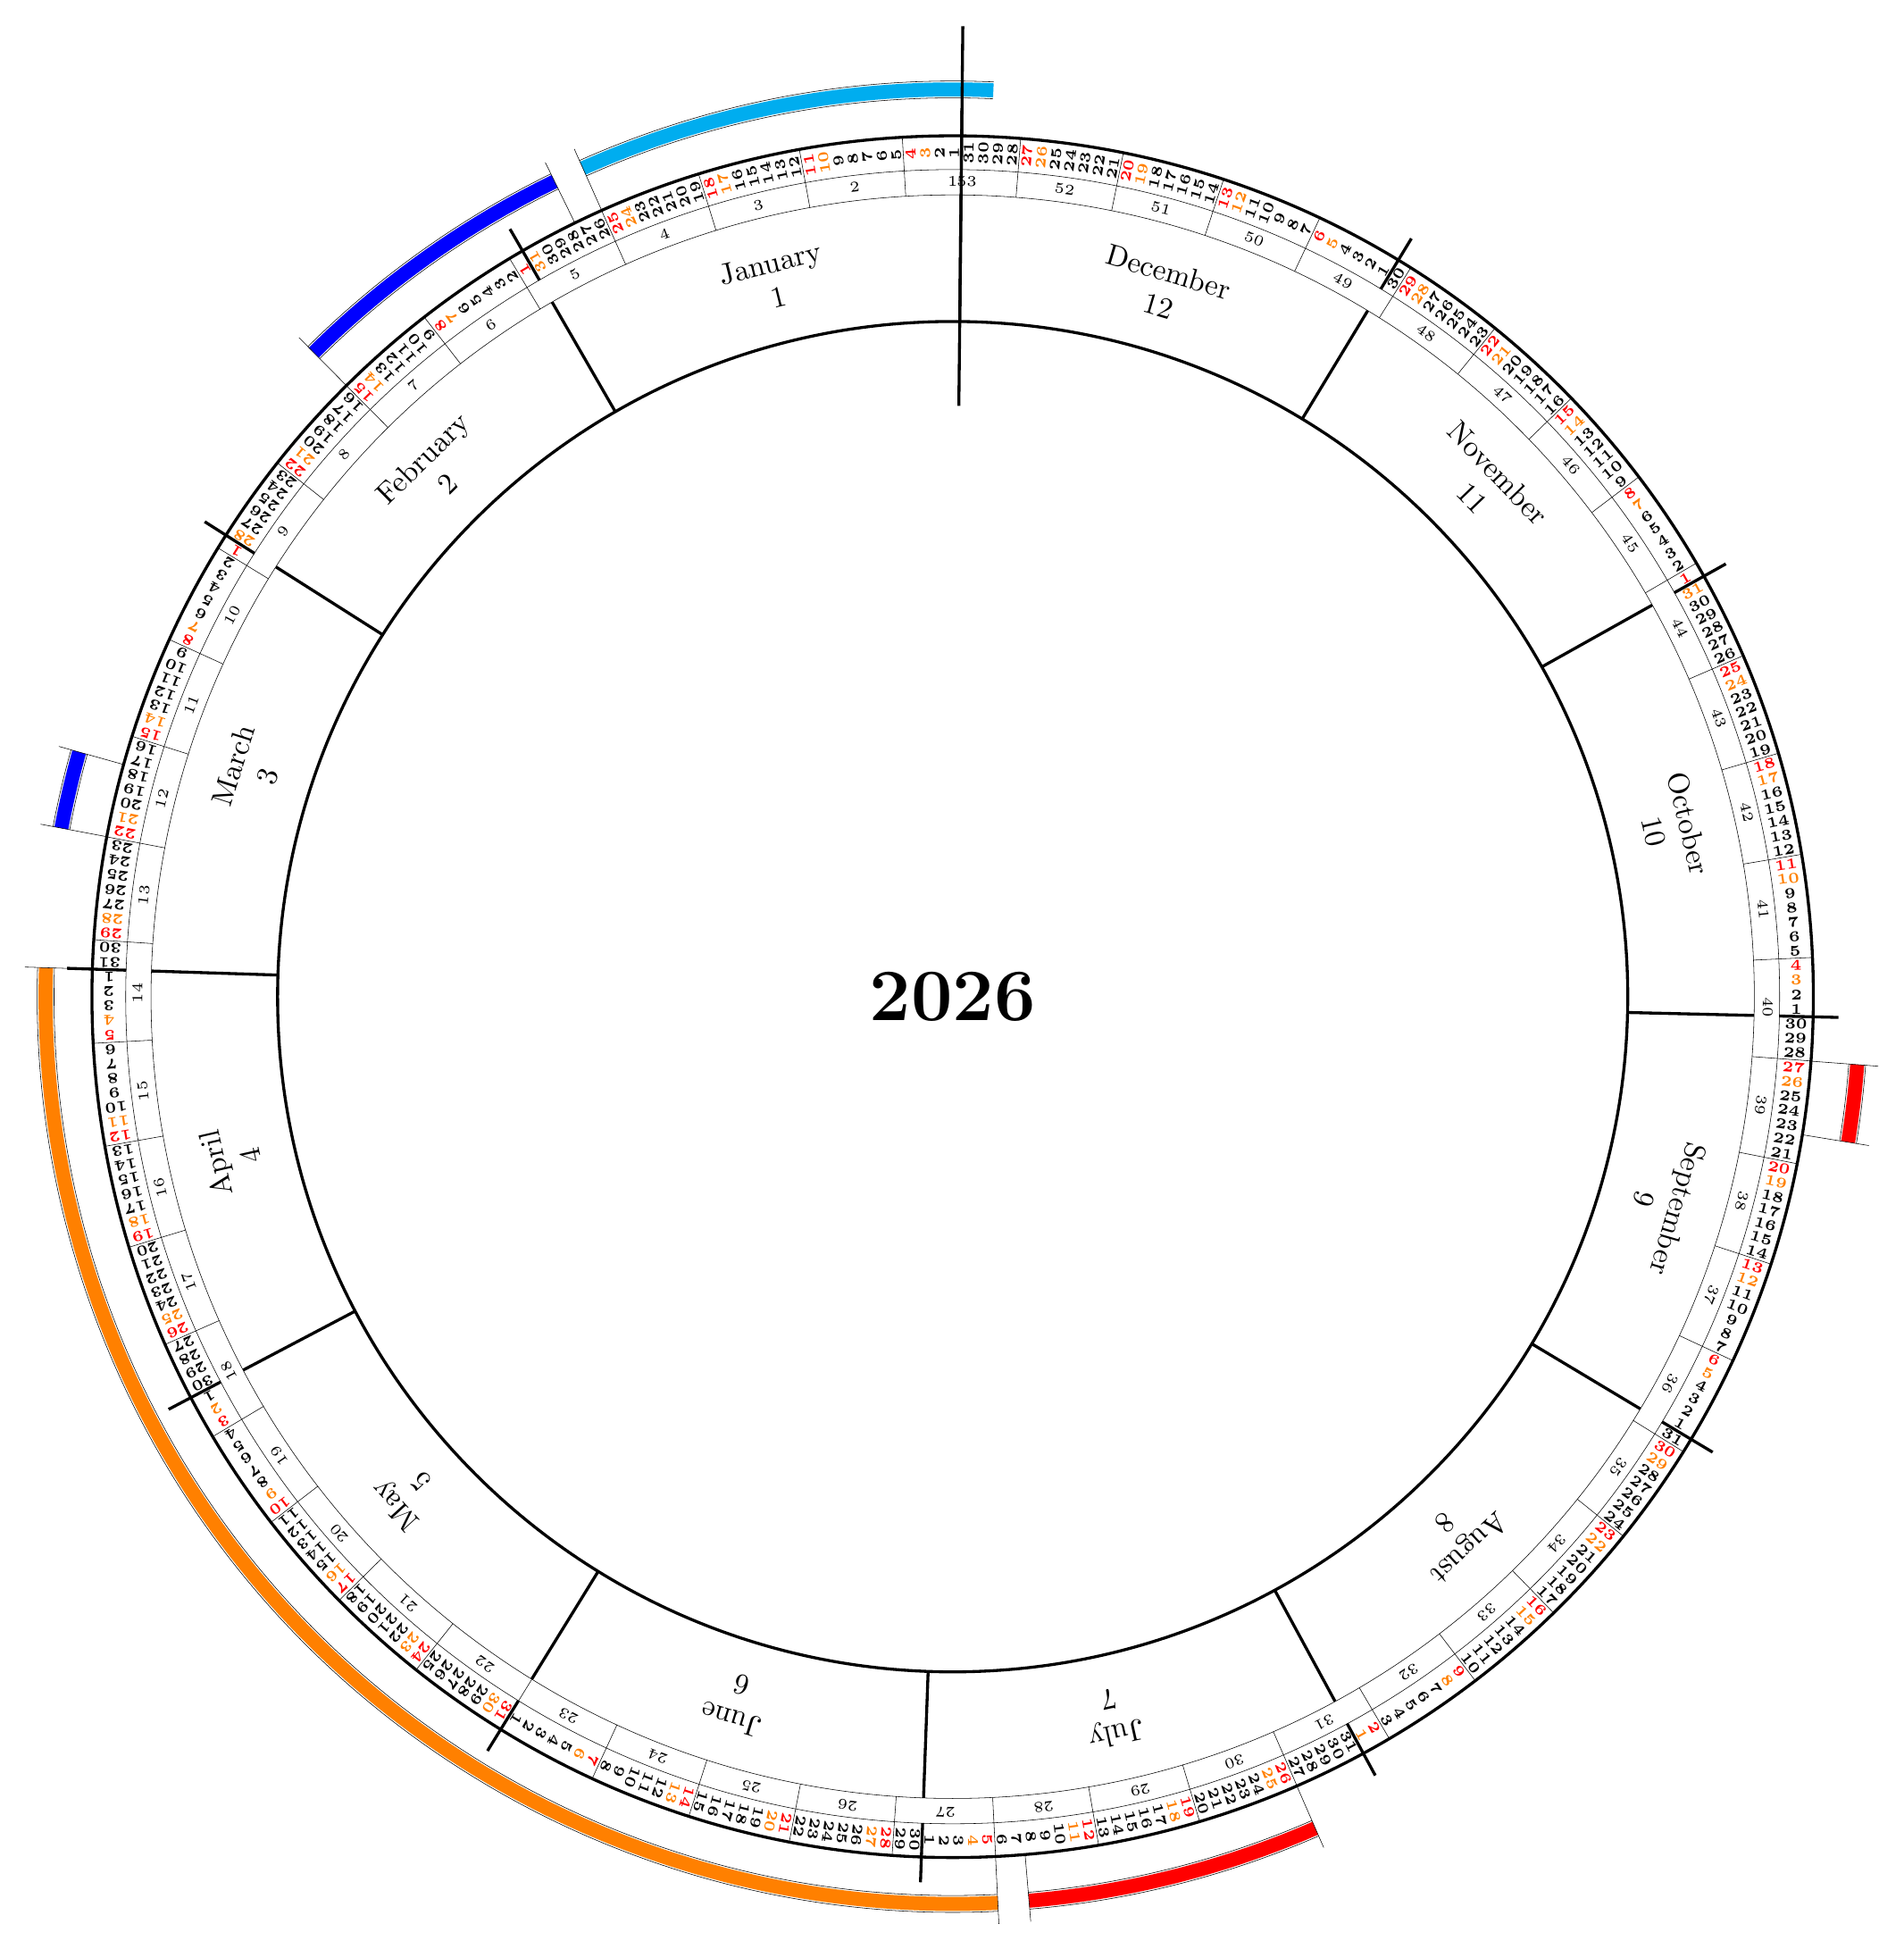
\begin{tikzpicture}[transform shape, every day/.style={anchor=mid, font=\bfseries\fontsize{4}{3}\selectfont, rotate=90 + \daycount  / 365 * 360}, scale=1.2]
    \daycount=0;
    \monthcount=0;
    \weekcount=1;
    \esose=0;
    % \advance\esose by \stopSoSe;

    \calendar at(0,0)[dates=\year-01-01 to \year-12-last, execute after day scope= {
      \advance\daycount by 1
      \ifdate{day of month=1} {%
        \advance\monthcount by 1
      }{}%
      \ifdate{Thursday} {%
        \advance\weekcount by 1
      }{}%
    }]
    if (Sunday) {
      \draw[very thin]
        let \n1 = {90 + \daycount / 365 * 360 + 0.4} in
      (\n1:9.5cm) -- (\n1:10.2cm);
      \tikzset{text=red}
    }
    if (Saturday) [orange]
    if (day of month=1) {
      \advance\monthcount by 1
      \draw
        let \n1 = {90 + \daycount / 365 * 360 + 14}
      in
        (\n1:8.75cm) node[align=center, text=black, rotate={\daycount / 365 * 360 + 14}] {\tikzmonthtext\\$\the\monthcount$};
      \draw[very thick]
        let \n1 = {90 + \daycount / 365 * 360 - 0.6}
      in
        (\n1:9.5cm) -- (\n1:8cm);
      \draw[very thick]
        let \n1 = {90 + \daycount / 365 * 360 - 0.6}
      in
        (\n1:9.8cm) -- (\n1:10.5cm);
    }
    if (Thursday) {
      \draw
        let \n1 = {90 + \daycount / 365 * 360}
      in
        (\n1:9.66cm) node[align=center, text=black, rotate={\daycount / 365 * 360}] {\tiny\the\weekcount};
    }
    if (all) {
      \pgftransformshift{\pgfpointpolar{90 + \daycount / 365 * 360}{10cm}}
    };
    \draw[very thick](0,0) circle (10.2cm);
    \draw[very thin](0,0) circle (9.8cm);
    \draw[very thin](0,0) circle (9.5cm);
    \draw[very thick](0,0) circle (8cm);

    \difftoday{2017}{04}{03}
    \ssose=\thedatetwo

    \difftoday{2017}{07}{08}
    \esose=\thedatetwo

    \difftoday{2017}{07}{10}
    \spasose=\thedatetwo

    \difftoday{2017}{07}{29}
    \epasose=\thedatetwo

    \difftoday{2017}{09}{25}
    \spbsose=\thedatetwo

    \difftoday{2017}{09}{30}
    \epbsose=\thedatetwo

    % sommersemester
    % vorlesungszeitraum
    \draw[line width = .2cm, color = orange]
    let
      \n1 = {90 + \ssose / 365 * 360 - 0.6},
      \n2 = {90 + \esose / 365 * 360 - 0.6}
    in
      (0,0) ++(\n1:10.75cm) arc (\n1:\n2:10.75cm);

    \draw[very thin]
    let
      \n1 = {90 + \ssose / 365 * 360 - 0.6},
      \n2 = {90 + \esose / 365 * 360 - 0.6}
    in
      (0,0) ++(\n1:10.85cm) arc (\n1:\n2:10.85cm);
    \draw[very thin]
    let
      \n1 = {90 + \ssose / 365 * 360 - 0.6},
      \n2 = {90 + \esose / 365 * 360 - 0.6}
    in
      (0,0) ++(\n1:10.65cm) arc (\n1:\n2:10.65cm);

    \draw[very thin]
      let \n1 = {90 + \ssose / 365 * 360 - 0.6}
    in
      (\n1:10.2cm) -- (\n1:11cm);

    \draw[very thin]
      let \n1 = {90 + \esose / 365 * 360 - 0.6}
    in
      (\n1:10.2cm) -- (\n1:11cm);

    % prüfungszeitraum 1
    \draw[line width = .2cm, color = red]
    let
      \n1 = {90 + \spasose / 365 * 360 - 0.6},
      \n2 = {90 + \epasose / 365 * 360 - 0.6}
    in
      (0,0) ++(\n1:10.75cm) arc (\n1:\n2:10.75cm);

    \draw[very thin]
    let
      \n1 = {90 + \spasose / 365 * 360 - 0.6},
      \n2 = {90 + \epasose / 365 * 360 - 0.6}
    in
      (0,0) ++(\n1:10.85cm) arc (\n1:\n2:10.85cm);
    \draw[very thin]
    let
      \n1 = {90 + \spasose / 365 * 360 - 0.6},
      \n2 = {90 + \epasose / 365 * 360 - 0.6}
    in
      (0,0) ++(\n1:10.65cm) arc (\n1:\n2:10.65cm);

    \draw[very thin]
      let \n1 = {90 + \spasose / 365 * 360 - 0.6}
    in
      (\n1:10.2cm) -- (\n1:11cm);

    \draw[very thin]
      let \n1 = {90 + \epasose / 365 * 360 - 0.6}
    in
      (\n1:10.2cm) -- (\n1:11cm);

    % prüfungszeitraum 2
    \draw[line width = .2cm, color = red]
    let
      \n1 = {90 + \spbsose / 365 * 360 - 0.6},
      \n2 = {90 + \epbsose / 365 * 360 - 0.6}
    in
      (0,0) ++(\n1:10.75cm) arc (\n1:\n2:10.75cm);

    \draw[very thin]
    let
      \n1 = {90 + \spbsose / 365 * 360 - 0.6},
      \n2 = {90 + \epbsose / 365 * 360 - 0.6}
    in
      (0,0) ++(\n1:10.85cm) arc (\n1:\n2:10.85cm);
    \draw[very thin]
    let
      \n1 = {90 + \spbsose / 365 * 360 - 0.6},
      \n2 = {90 + \epbsose / 365 * 360 - 0.6}
    in
      (0,0) ++(\n1:10.65cm) arc (\n1:\n2:10.65cm);

    \draw[very thin]
      let \n1 = {90 + \spbsose / 365 * 360 - 0.6}
    in
      (\n1:10.2cm) -- (\n1:11cm);

    \draw[very thin]
      let \n1 = {90 + \epbsose / 365 * 360 - 0.6}
    in
      (\n1:10.2cm) -- (\n1:11cm);


    % wintersemester 2016/2017
    % vorlesungszeitraum
    \difftoday{2017}{01}{01}
    \swise=\thedatetwo

    \difftoday{2017}{01}{28}
    \ewise=\thedatetwo

    \difftoday{2017}{01}{30}
    \spawise=\thedatetwo

    \difftoday{2017}{02}{18}
    \epawise=\thedatetwo

    \difftoday{2017}{03}{20}
    \spbwise=\thedatetwo

    \difftoday{2017}{03}{25}
    \epbwise=\thedatetwo

    \draw[line width = .2cm, color = cyan]
    let
      \n1 = {90 + \swise / 365 * 360 - 0.6},
      \n2 = {90 + \ewise / 365 * 360 - 0.6}
    in
      (0,0) ++(\n1:10.75cm) arc (\n1:\n2:10.75cm);

    \draw[very thin]
    let
      \n1 = {90 + \swise / 365 * 360 - 0.6},
      \n2 = {90 + \ewise / 365 * 360 - 0.6}
    in
      (0,0) ++(\n1:10.85cm) arc (\n1:\n2:10.85cm);
    \draw[very thin]
    let
      \n1 = {90 + \swise / 365 * 360 - 0.6},
      \n2 = {90 + \ewise / 365 * 360 - 0.6}
    in
      (0,0) ++(\n1:10.65cm) arc (\n1:\n2:10.65cm);

    % \draw[very thin]
    %   let \n1 = {90 + \swise / 365 * 360 - 0.6}
    % in
    %   (\n1:10.2cm) -- (\n1:11cm);

    \draw[very thin]
      let \n1 = {90 + \ewise / 365 * 360 - 0.6}
    in
      (\n1:10.2cm) -- (\n1:11cm);

    % prüfungszeitraum 1
    \draw[line width = .2cm, color = blue]
    let
      \n1 = {90 + \spawise / 365 * 360 - 0.6},
      \n2 = {90 + \epawise / 365 * 360 - 0.6}
    in
      (0,0) ++(\n1:10.75cm) arc (\n1:\n2:10.75cm);

    \draw[very thin]
    let
      \n1 = {90 + \spawise / 365 * 360 - 0.6},
      \n2 = {90 + \epawise / 365 * 360 - 0.6}
    in
      (0,0) ++(\n1:10.85cm) arc (\n1:\n2:10.85cm);
    \draw[very thin]
    let
      \n1 = {90 + \spawise / 365 * 360 - 0.6},
      \n2 = {90 + \epawise / 365 * 360 - 0.6}
    in
      (0,0) ++(\n1:10.65cm) arc (\n1:\n2:10.65cm);

    \draw[very thin]
      let \n1 = {90 + \spawise / 365 * 360 - 0.6}
    in
      (\n1:10.2cm) -- (\n1:11cm);

    \draw[very thin]
      let \n1 = {90 + \epawise / 365 * 360 - 0.6}
    in
      (\n1:10.2cm) -- (\n1:11cm);

    % prüfungszeitraum 2
    \draw[line width = .2cm, color = blue]
    let
      \n1 = {90 + \spbwise / 365 * 360 - 0.6},
      \n2 = {90 + \epbwise / 365 * 360 - 0.6}
    in
      (0,0) ++(\n1:10.75cm) arc (\n1:\n2:10.75cm);

    \draw[very thin]
    let
      \n1 = {90 + \spbwise / 365 * 360 - 0.6},
      \n2 = {90 + \epbwise / 365 * 360 - 0.6}
    in
      (0,0) ++(\n1:10.85cm) arc (\n1:\n2:10.85cm);
    \draw[very thin]
    let
      \n1 = {90 + \spbwise / 365 * 360 - 0.6},
      \n2 = {90 + \epbwise / 365 * 360 - 0.6}
    in
      (0,0) ++(\n1:10.65cm) arc (\n1:\n2:10.65cm);

    \draw[very thin]
      let \n1 = {90 + \spbwise / 365 * 360 - 0.6}
    in
      (\n1:10.2cm) -- (\n1:11cm);

    \draw[very thin]
      let \n1 = {90 + \epbwise / 365 * 360 - 0.6}
    in
      (\n1:10.2cm) -- (\n1:11cm);



    \node[font=\fontsize{100}{45}\selectfont] at (0,0){$\bf\the\year$};

    \draw[very thick]
      let \n1 = {90 + 0 / 365 * 360 - 0.6}
    in
      (\n1:7cm) -- (\n1:11.5cm);
  \end{tikzpicture}
\end{document}
